% !TEX root = diplomarbeit.tex
\chapter{Mechanik}

\renewcommand{\kapitelautor}{Autor: Alexander Punz}

\section{Allgemeine technische Planung}

		\subsubsection{Allgemeine Informationen über 3D Drucken}

		Die Technologie des 3D Druckens hat in den letzten Jahren immer mehr an Popularität gewonnen. Mit Hilfe des 3D Druckers kann man fast alle vorstellbaren Formen anfertigen.
		Es gibt verschiedenste Verfahren wie man ein Werkstück anfertigen kann: Laser Sintern, Stereolithographie, Drucken mit flüssigen Materialien, etc.
		In diesem Projekt wird nur die Variante des Druckens mit flüssigen Material verwendet.
		Diese ist kostengünstig \bzw genau genug für die Teile. Wie der Name schon sagt, wird Material in einem Druckkopf geschmolzen und dann Schicht für Schicht auf der Druckplatte aufgetragen.
		Der Druckkopf fährt nur in X und Y Richtung, die Höhe wird mit der Druckplatte selbst verfahren.

		Meist werden Drucker über einen Maschinencode gesteuert, dem sogenannten „G-Code“. In diesem Code werden die Punkte (Koordinaten) definiert, die der Extruder (Druckkopf) abfahren muss.
		Die folgende Abbildung zeigt ein Beispiel eines Maschinencodes.

			\begin{figure}[tbh]
			\begin{centering}
			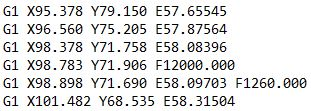
\includegraphics[width = 0.45\textwidth]{Bilder/gcode_erklaerung}
			\par\end{centering}
			\caption{Maschinencode Erklärung}
			\label{gcode_erklaerung}
			\end{figure}

			% Table generated by Excel2LaTeX from sheet 'Tabelle1'
			\begin{table}[htbp]
  		\centering
  		\caption{Befehle G Code}
	    \begin{tabular}{ll}
	    G1    & Kontrollierte Bewegung \\
	    X, Y  & Koordinaten in horizontaler und vertikaler Richtung \\
	    E     & Angabe der Menge des Filaments, dass in den Extruder geschoben werden muss \\
	    F     & Geschwindigkeit, mit der das Material in den Extruder geschoben wird (mm/min) \\
	    \end{tabular}%
	  	\label{tab:befehle gcode}%
			\end{table}%

		Je nachdem wie der Drucker aufgebaut ist, werden die Produkte genau oder nur grob angefertigt. Sehr genaue Teile kann man am besten in einem Drucker produzieren, der einen geschlossenen Druckraum \bzw eine beheizte Druckplatte hat.
		Besonders an dünnen Platten merkt man das. Wenn der Druckraum nach \bzw während des Druckvorgangs warm ist, kühlt das Werkstück an jeder Stelle fast gleich ab.
		Ist der Druckraum offen, kühlt das Werkstück in der Mitte schneller ab, kühles Material zieht sich zusammen, daher biegt sich das Material auf.

			\newpage

		Es kann vorkommen, dass ein Teil nur so gedruckt werden kann, wenn es nicht komplett auf der Druckplatte aufliegt zum Beispiel ein Steg, der „in der Luft“ liegt oder eine Bohrung im Werkstück, die horizontal gedruckt werden muss.
		In solchen Fällen, druckt der Drucker unter diesem Steg Stützmaterial. Basierend auf diesem Stützmaterial, wird dann die gewünschte Form gedruckt.
		Das Stützmaterial ist so gefertigt, dass man es leicht von dieser abbrechen kann, ohne dass Rückstände zurück bleiben.

		\subsubsection{Materialeigenschaften}

		\subsubsection{Von der Idee zur Anfertigung}

		Die größte Hürde an der Realisierung einer Idee ist, eine CAD Zeichnung zu erstellen. In 3D CAD Programmen wie Creo, SolidWorks, etc. kann man ein Teil konstruieren und dann als STL (Standard Triangulation Language) File abspeichern.
		Dieses Format gibt dann nur mehr Informationen über die Oberfläche und Struktur an (siehe Abbildung\ref{stl_file_optionen}).
		Die Sehnenhöhe gibt an wie genau die Oberfläche gedruckt werden muss, die Winkelsteuerung gibt die Genauigkeit der Radien und Kanten des Teiles an.


			\begin{figure}[tbh]
			\begin{centering}
			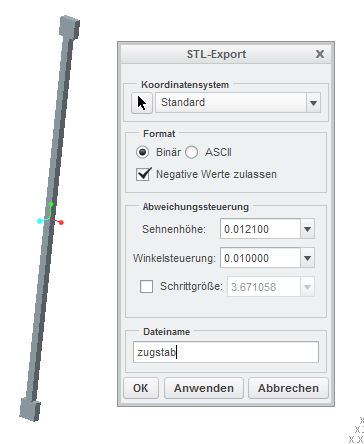
\includegraphics[width = 0.5\textwidth]{Bilder/stl_file_optionen}
			\par\end{centering}
	 		\caption{Einstellung für STL File}
			\label{stl_file_optionen}
			\end{figure}

		Mit diesem File kann man anschließend in Programmen wie Slic3r den gewünschten Maschinencode generieren lassen.
		In diesen Programmen gibt man die Lage des Werkstückes an \bzw in genaueren Einstellungen auch die Temperatur des Druckbettes, den Geschwindigkeiten und ähnliche Konfigurationen.

		Am häufigsten haben die Drucker eine USB Schnittstelle, \bzw verfügen über einen SD Karten Slot.
		Der Maschinencode wird auf diesen Speichermedien gespeichert und einfach auf den Drucker überspielt.


\section{Halterung für Cupcakes}

		\subsection{Technische Planung}

		Die Diplomarbeit hat sich speziell auf den Transport von Cupcakes spezialisiert, um diesen sicher transportieren zu können, ist es notwendig eine Halterung zu konzipieren.
		Zu beachten ist, dass die Halterung möglichst wenig wiegt \bzw leicht zu montieren ist.

		Der Akku wurde an der Unterseite des Hexacopters befestigt, daher war es nur mehr möglich die Halterung an der oberen Centerplate zu platzieren.
		Damit der Multicopter möglichst ausgewogen ist, muss sich das zu transportierende Objekt in der Mitte befinden.
		Die Idee war es daher, den Cupcake mit einer Halterung zu umranden, um ihn gegen Verrutsche zu sichern. Die Geometrie der Platte \bzw die Größe des Objektes hat die Befestigungsmöglichkeiten etwas eingeschränkt (siehe Abbildung \ref{platte_cupcake}).
		Die innere Reihe der Langlöcher würde sich optimal anbieten, um die Halterung befestigen zu können, die Cupcakeform kann so direkt von einer Haltevorrichtung gestützt werden.


			\begin{figure}[tbh]
			\begin{centering}
			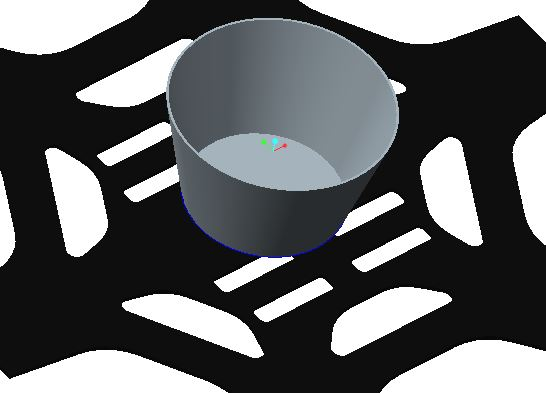
\includegraphics[width = 0.5\textwidth]{Bilder/platte_cupcake}
			\par\end{centering}
			\caption{Position Cupcake}
			\label{platte_cupcake}
			\end{figure}

			\newpage

	\subsection{Umsetzung}

	Wie schon in der technischen Planung erwähnt wurde, sollte der Cupcake von einer Haltevorrichtung umrandet werden.
	Die inneren Ausnehmungen der oberen Centerplate haben sich optimal angeboten, da diese direkt bis zur Form reichen.

	Es wurden Stützen konstruiert, die in den Ausnehmungen fixiert werden können und sich direkt an das Dessert anpassen.
	Die folgenden Abbildungen zeigen die konstruierten Halterungsstutzen und deren Befestigung.

			\begin{figure}[H]
			  \begin{centering}
			    \subfigure[Halterung Cupcake oben\label{halterung_cupcake_oben_grosz}]{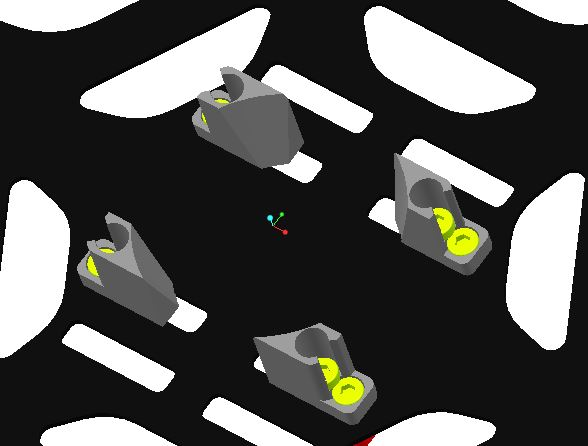
\includegraphics[width = 0.4\textwidth]{Bilder/halterung_cupcake_oben_grosz}}
			    \subfigure[Halterung Cupcake unten\label{halterung_cupcake_unten_grosz}]{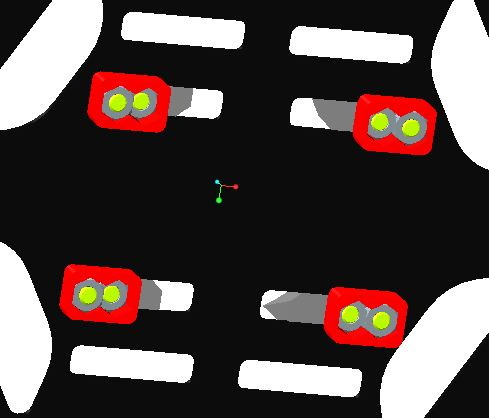
\includegraphics[width = 0.4\textwidth]{Bilder/halterung_cupcake_unten_grosz}}
			  \par\end{centering}
			  \caption{Halterung Cupcake}
			  \label{Halterung_Cupcake}
			\end{figure}

	Die Stützen (siehe Abbildung \ref{halterung_cupcake_oben_grosz}) wurden so entworfen, dass sie sich dem Radius \bzw der Höhe der Form des Cupcake anpassen.
	Die Höhe der Halterung wurde so gewählt, dass etwa die Hälfte der Cupcakeform frei liegt.
	Das soll vermeiden, dass man sich die Finger beim Entnehmen des Cupcakes an der Creme schmutzig macht.

	Die Halterung wird direkt an der Centerplate mit Durchgangsschrauben und Muttern festgeschraubt.
	Durch den Platzmangel mussten M4 Schrauben gewählt werden, da diese klein sind und trotzdem viel Beanspruchung aufnehmen können.
	Die Schlüsselweite einer M4 Mutter beträgt 7.0 mm, die Breite der Ausnehmung 6.5 mm, würde man die Schrauben direkt mit der Platte verschrauben, müsste man eine Beilagscheibe zwischenlegen, um eine größere Aufliegefläche für die Mutter zu erhalten.

	Es wurden spezielle Mutterhalter entworfen (siehe Abbildung \ref{halterung_cupcake_unten_grosz}), diese bezwecken zwei Funktionen:
	Einerseits muss man die Muttern während man die Halterung montiert nicht mehr festhalten und andererseits kann man die Schraubenverbindung viel fester anziehen, da man die Platte nicht mehr beschädigen kann.

	Der Platz für die Stutzen entlang der Langlöcher ist nur so kurz, dass sich die Köpfe der Schrauben und die Muttern schneiden würden.
	Um dieses Problem zu beheben, wurden Höhenunterschiede zwischen den Schrauben eingeplant.
	Das macht die Halterungsstutzen kompakter und verhindert Kollisionen.

		\newpage

	\subsection{Herausforderungen und Lösungen}

	Die größte Herausforderung beim Konstruieren war es, die Halterung an die Form des Cupcakes anzupassen.
	Die Halterungsstützen sollen an die Rundung \bzw den Durchmesserverlauf der Cupcakeform angepasst werden.
	Um die richtige Form der Stützen konstruieren zu können, wurde erst der Winkel der Cupcakeform mit der  folgenden Formel ermittelt:

			\begin{figure}[tbh]
			\begin{centering}
			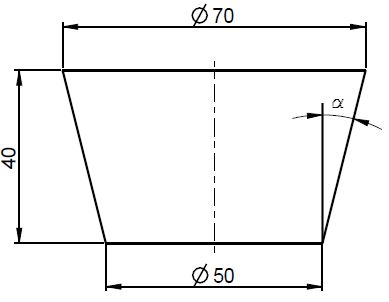
\includegraphics[width = 0.4\textwidth]{Bilder/berechnung_winkel}
			\par\end{centering}
			\caption{Berechnung des Winkels}
			\label{berechnung_winkel}
			\end{figure}

			\begin{align}
 				\tan x = \frac{35mm-25mm}{40mm}  \qquad \alpha = \arctan \frac{35mm-25mm}{40mm} = 14.04^\circ
 			\end{align}

	Konstruiert wurde die Halterung mit einem Winkel von 15° um Ungenauigkeiten des Druckers besser kompensieren zu können.
	In der folgenden Abbildung kann man erkennen, dass manche Wände bei den Bohrungen zu dünn sind zu drucken, es entstehen dadurch Löcher.
	Dieses Problem könnte man nur lösen, wenn man die Schrauben weiter nach außen legen würde, jedoch ist das in diesem Fall nicht möglich, da die Ausnehmungen zu kurz sind.


			\begin{figure}[tbh]
			\begin{centering}
			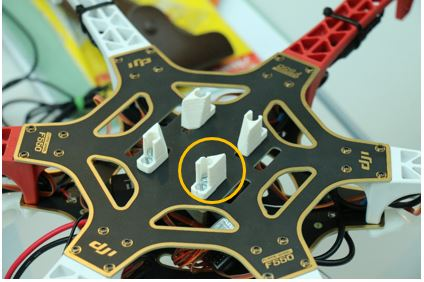
\includegraphics[width = 0.65\textwidth]{Bilder/halterung_cupcake_fertig_hinweis}
			\par\end{centering}
			\caption{Gedrucktes Halterungssystem}
			\label{halterung_cupcake_fertig_hinweis}
			\end{figure}

\section{Rotorschutz}

	\subsection{Technische Planung}

	\subsection{Umsetzung}

	\subsection{Herausforderungen und Lösungen}

	\subsection{Implementierung}

\section{Halterung Ultraschallsensor}

	\subsection{Technische Planung}

	\subsection{Umsetzung}

	\subsection{Herausforderungen und Lösungen}

\section{Halterung PIXY CMU cam5}

	\subsection{Technische Planung}

		\subsubsection{Berechnungen}

	\subsection{Umsetzung}

	\subsection{Implementierung}

	\subsection{Testphase}

\section{Führung für Testflüge}

	\subsection{Technische Planung}

	\subsection{Umsetzung}

	\subsection{Implementierung}

	\subsection{Testphase}

\section{Persönliche Erfahrungen}
